\documentclass[10pt,a4paper]{article}
\usepackage[utf8]{inputenc}
\usepackage[czech]{babel}
\usepackage{amsmath}
\usepackage{amsfonts}
\usepackage{amssymb}
\usepackage{chemfig}
\usepackage{geometry}
\usepackage{wrapfig}
\usepackage{graphicx}
\usepackage{floatflt}
\usepackage{hyperref}
\renewcommand{\labelitemii}{$\circ$}
\renewcommand{\labelitemiii}{--}
\newcommand{\ra}{$\rightarrow$ }
\geometry{lmargin = 0.8in, rmargin = 0.8in, tmargin = 0.8in, bmargin = 0.8in}
\title{Střední Evropa}
\date{\today}
\author{Jakub Rádl}
\begin{document}
\maketitle
\tableofcontents
\newpage
\mbox{}
\vspace{-1.5cm}
\begin{wrapfigure}{r}{3cm}
\frame{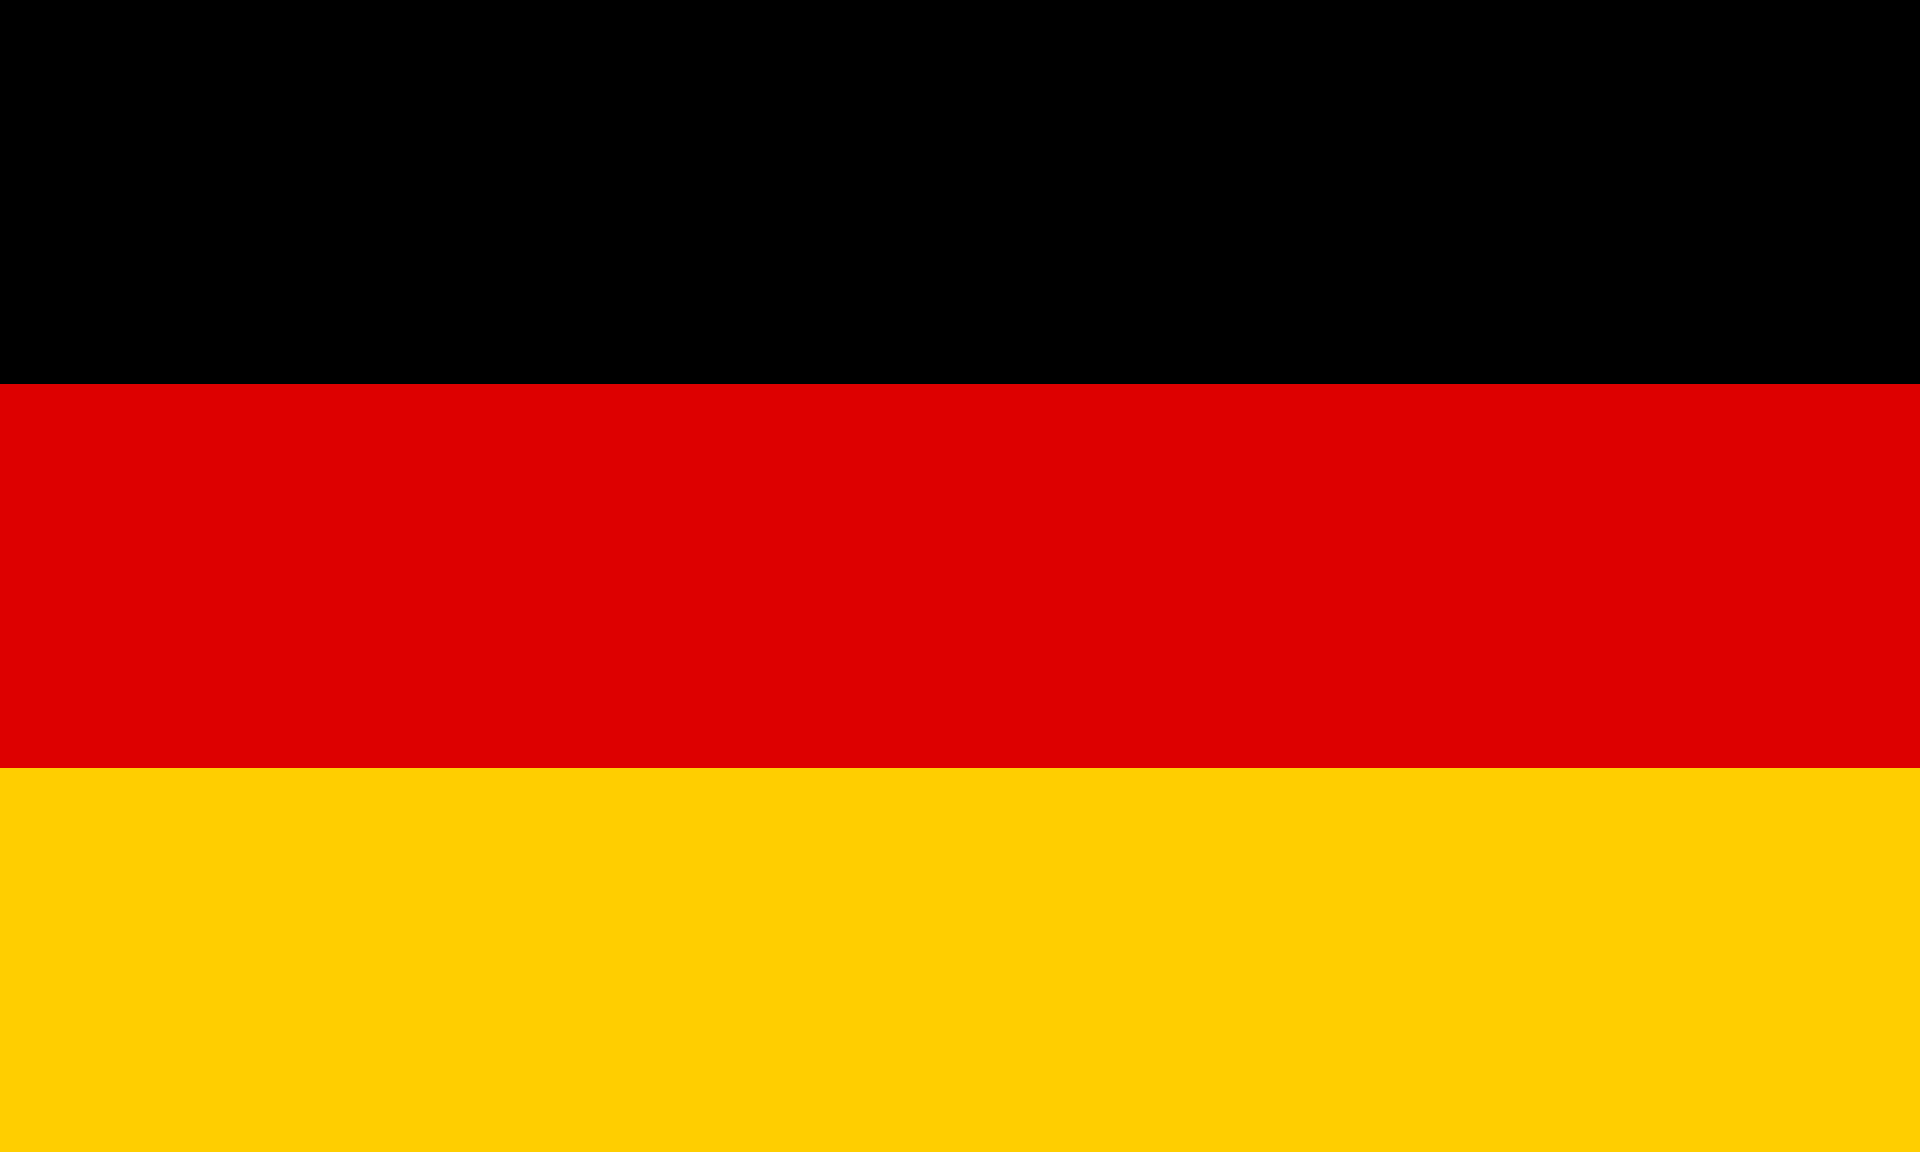
\includegraphics[height=2cm]{pictures/flag_DE.png}}
\vspace{-200pt}
\end{wrapfigure}
\section{Německo}



\newpage
\mbox{}
\vspace{-1.5cm}
\begin{wrapfigure}{r}{3cm}
\frame{
\includegraphics[height=2cm]{pictures/flag_A.png}}
\vspace{-200pt}
\end{wrapfigure}
\section{Rakousko}



\newpage
\mbox{}
\vspace{-1.5cm}
\begin{wrapfigure}{r}{3cm}
\frame{
\includegraphics[height=2cm]{pictures/flag_CH.png}}
\vspace{-200pt}
\end{wrapfigure}
\section{Švýcarsko}



\newpage
\mbox{}
\vspace{-1.5cm}
\begin{wrapfigure}{r}{3cm}
\frame{
\includegraphics[height=2cm]{pictures/flag_PL.png}}
\vspace{-200pt}
\end{wrapfigure}
\section{Polsko}
\subsection{Přírodní podmínky}
\paragraph{Otázečky}
\begin{enumerate}
\item Vyhledej na mapě: Pomořanská, Mazurská jezerní plošina; Velkopolská, Slezská, Mazovská nížina; Lublinská, Malopolská vrchovina; pohraniční pohoří s Českem a Slovenskem; Bělověřský prales; řeky Visla, Odra, Varta; jezero Sinardwy
\end{enumerate}

\paragraph{Povrch}
\begin{itemize}
\item většina povrchu -- \textbf{nížiny} a ledovcové \textbf{jezerní plošiny}
\item v jižní části vrchoviny, na hranici s ČR a SR pohoří
\item nížiny kolem Baltského moře ( ... )
\item přechod kontinentálního klimatu od severu k jihu
\end{itemize}

\paragraph{Vodstvo}
\begin{itemize}
\item většina řek je odvodňována do \textbf{Baltského moře}
\item \textbf{Sinardwy} -- největší jezero, v Mazurské plošině
\item \textbf{Helská kosa} (kosa = pruh pevniny nanesený mořskými proudy)
\end{itemize}

\paragraph{Běloveský národní park}
\begin{itemize}
\item na Hranici s Běloruskem
\item populace \textbf{zubra evropského}, divokých koňů (tarpanů)
\item nížinný typ pralesa s převahou listnatých dřevin (staleté duby)
\end{itemize}

\paragraph{Sloviňský národní park}
\begin{itemize}
\item na pobřeží Baltu
\item pohyblivé \textbf{písečné duny}
\item jezera občas sycená mořskou vodou (při bouřích) \ra výskyt \textbf{halofytních} (slanomilných) druhů (los, bobr, tuleň, sviňucha)
\end{itemize}


\subsection{Historie, obyvatelstvo, administrativní členění}
\paragraph{Otázečky}
\begin{enumerate}
\item Na mapách v atlase (\textit{str. 52, 53}) a pomocí textu v učebnici (\textit{str. 32}) vyhodnoť územní změny v Polsku
\end{enumerate}

\paragraph{Historie}
\begin{itemize}
\item polsko-litevské knížectví
\item německá kolonizace severu a západu
\item trojí dělení Polska
\item změna hranic po 2. sv. válce
\item Varšava po 2. sv. válce zničena (v nedávné době obnovena)
\item vyvraždění důstojníků polské armády Sověty
\end{itemize}

\paragraph{Obyvatelstvo}
\begin{itemize}
\item 38 milionů obyvatel
\item husté osídlení jihu v pásu od Wroclavi po Katovice (výskyt surovin $\rightarrow$ průmysl)
\item k hlavním centrům patří Vršava, Poznaň, Lódž, Vroclav, Katovice, Krakov, Gdaňsk, Štětín
\item \textbf{rozdíly v životní úrovni} ve městech a na venkově
\item rozdíly mezi vyspělostí západu a východu
\end{itemize}

\paragraph{Administrativní členění}
\begin{itemize}
\item členěno na \textbf{vojvodství} (ekvivalent českých krajů)
\end{itemize}

\paragraph{Významná města}
\begin{itemize}
\item \textbf{Gdaňsk} -- přístav
\item \textbf{Malbork} -- křižácká pevnost
\item \textbf{Krakov} -- ve své době sídlem králů, hrad Wawel
\item \textbf{Lešno} -- shořely zde spisy J. A. Komenského
\item \textbf{Toruň} -- rodiště Mikoláše Koperníka (autor heliocentrického světového názoru)
\item \textbf{Osvětim-Březinka} -- koncentrační tábor
\item \textbf{Wieliczka} -- solné doly (těžba ukončena, ze soli vytesané sochy)
\item \textbf{Zakopane} -- lyžařské středisko
\end{itemize}


\subsection{Ekonomika}
\begin{itemize}
\item člen EU
\item zásoby \textbf{surovin} na jihu (uhlí, síra, zinek, měď)
\item průmysl soustředěný v oblasti \textbf{Horno a Dolnoslezské pánve}
\item těžba a průmysl se projevuje na životním prostředí $\rightarrow$\textbf{ útlum a restrukturalizace} těžkého průmyslu
\end{itemize}

\paragraph{Zemědělství}
\begin{itemize}
\item velká zemědělská produkce
\item stále \textbf{vysoký podíl pracujících v zemědělství} (cca 12%)
\item významná \textbf{produkce žita, lnu, brambor, cukrové řepy a masa}
\end{itemize}

\paragraph{Katovická aglomerace (konurbace)}
\begin{itemize}
\item \textbf{největší} aglomerace ve \textbf{východní části střední Evropy}
\item problémy s útlumem těžkého průmyslu
\item města: Katovice, Sosnowiec, Gliwice, Chorzow
\item největší síť tramvajové dopravy na světě (spojuje města)
\end{itemize}



\newpage
\mbox{}
\vspace{-1.5cm}
\begin{wrapfigure}{r}{3cm}
\frame{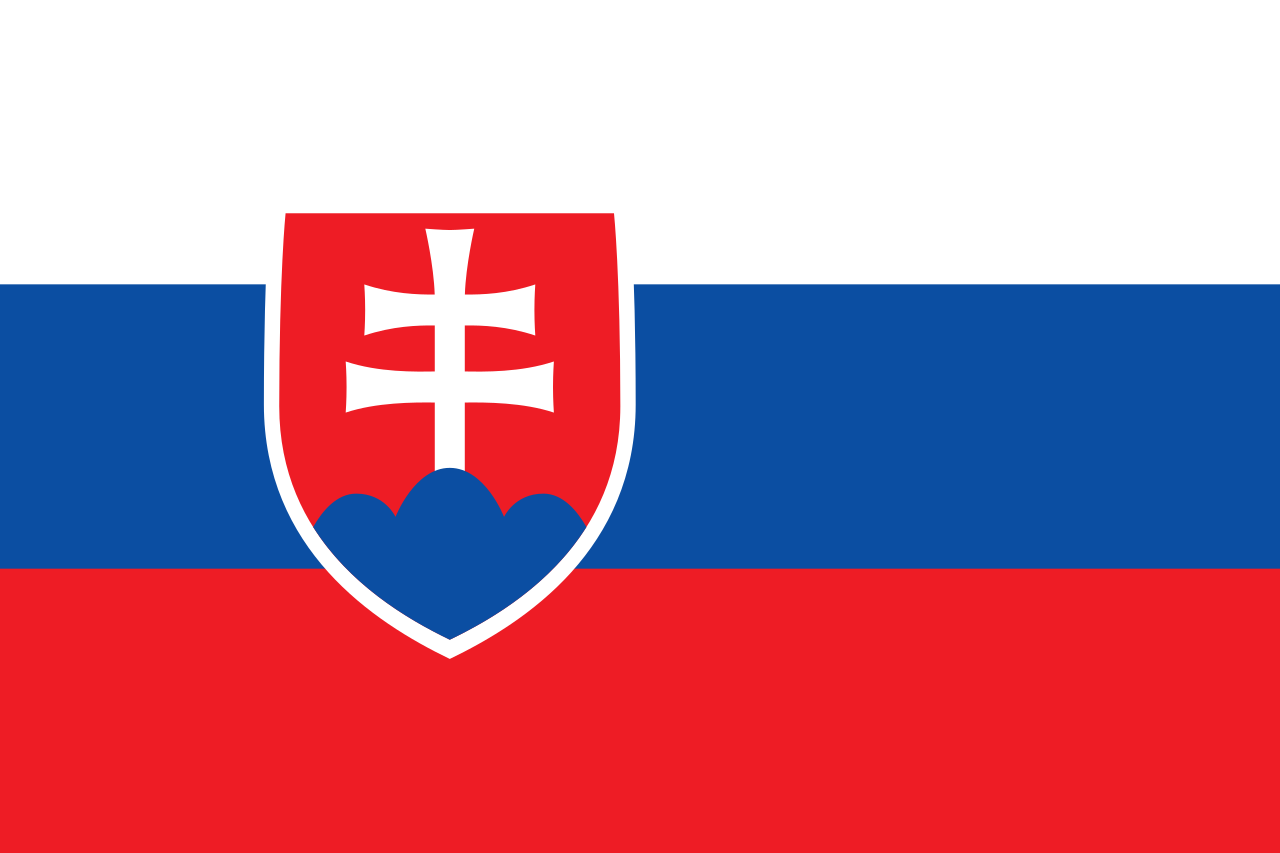
\includegraphics[height=2cm]{pictures/flag_SK.png}}
\vspace{-200pt}
\end{wrapfigure}	
\section{Slovensko} 
\subsection{Karpatský oblouk}
\begin{itemize}
\item pásemné pohoří táhnoucí se cca \textbf{1500km}
\item táhne se přes konec Rakouska, bok ČR, \textbf{Slovensko}, jih Polska, \textbf{Ukrajinu}, \textbf{Rumunsko}, sever Srbska
\item v pleistocénu zalednění nejvyšších oblastí, dnes jen pozůstalé ledovcové útvary
\item dělení
\begin{itemize}
\item Západní (\textbf{Gerlachovský štít} -- 2655, Slovensko)
\item Východní (\textbf{Pietrosul} -- 2303, Rumunsko)
\item Jižní (\textbf{Moldoveanu} -- 2543, Ukrajina)
\end{itemize}
\item horninový poklad tvořen flyšovým pásmem (pískovce, břidlice), krystalickými horninami (žula), vápenci a vulkanickými horninami
\begin{itemize}
\item vnější Karpaty -- pískovce, břidlice
\item vnitřní Karpaty -- pevné krystalické horniny
\end{itemize}
\item rozsáhlé plochy lesních porostů, velká populace vlků a medvědů
\end{itemize}


\subsection{Přírodní podmínky}
\begin{itemize}
\item většinu území zabírají \textbf{Karpaty} (flyšové a centrální pásmo -- vnější a vnitřní západní Karpaty)
\item nejvyšší pohoří
\begin{itemize}
\item \textbf{Tatry} (\textbf{Gerlachovský štít} -- 2655)
\item \textbf{Nízké Tatry} (\textbf{Ďumbier} -- 2043, Chopok)
\end{itemize}
\item třetí nejzalesněnější stát Evropy
\item soustava horských kotlin -- Liptovská + Popradská (Podtatranská), Turčianská (mezi Malou a Velkou Fatrou), Horehronská
\item množství národních parků (TANAP, NAPANT, Pieniny, Malá Fatra, Slovenský kras)
\item výběžky Panonské pánve -- Podunajská a Východoslovenská nížina
\item řeky Dunaj, Váh, Nitra, Hron (všechny na jihozápadě vtékají do Dunaje)
\begin{itemize}
\item \textbf{Dunaj}
\begin{itemize}
\item velké říční přístavy v Bratislavě a Komárně
\item Malý Dunaj -- rameno Dunaje odpojující se v Bratislavě a vracející se v Komárně
\item přehrada Gabčíkovo
\end{itemize}
\item \textbf{Váh}
\end{itemize}
\end{itemize}


\paragraph{Tatry}
\begin{itemize}
\item nejvyšší pohoří Slovenska a Karpat
\item rozdělení na \textbf{Západní} (Roháče), \textbf{Východní} (Vysoké a Belanské)
\item jsou součástí TANAPu, který je v seznamu UNESCO
\item nejznámější vrcholy: Gerlach, Kriváň, Vysoká, Lomnický štít, Rysy, Slavkovský štít
\item pramen Bieleho Váhu
\item od Nízkých Tater je pohoří odděleno Podtatranskou kotlinou s Liptovskou Mašou
\end{itemize}

\paragraph{Pieniny}
\begin{itemize}
\item \textbf{národní park} na hranici Slovenska s Polskem
\item pohoří tvořeno převážně jurskými a křídovými \textbf{vápenci}
\item hluboké \textbf{údolí a soutěsky} vymodelované řekou \textbf{Dunajec}
\item vrchol \textbf{Trzy Korony} s pěti skalními věžemi (až 100m)
\item vodáctví na Dunajci
\begin{itemize}
\item \textbf{pltě} -- dřevěné rafty
\end{itemize}
\end{itemize}

\paragraph{Slovenský kras}
\begin{itemize}
\item největší krasové území na Slovensku ($>$ 400 km$^2$), UNESCO
\item rozkládá se na hranici s Maďarskem
\item náhorní planiny, závrty, propasti, jeskyně, \ldots
\item jeskyně \textbf{Domica}
\begin{itemize}
\item státní hranice
\item největší známý stalagmit na světě (25m)
\end{itemize}
\end{itemize}


\subsection{Historie, sociální prostředí}
\paragraph{Otázečky}
\begin{enumerate}
\item Vyhledej v atlase: Košice, Žilina, Poprad, Banská Bystrica, Trenčín, Trnava, Nitra, Zvolen, Banská Šťiavnica, Vlkolínec, Bardejov, Spišský hrad
\item Seznamte se s administrativním členěním Slovenska
\end{enumerate}

\paragraph{Historie}
\begin{itemize}
\item 900 let součástí uher
\item 1918 -- vznik Československa
\item vyhlášení Slovenského štátu 1939-1945
\item 1993 -- Slovenská republika
\end{itemize}


\end{document}
